\section{Các Kiến trúc kinh điển: AlexNet và VGG}
\label{sec:classic_architectures}

Nếu các thành phần cơ bản trong phần trước là những nốt nhạc riêng lẻ, thì phần này là nơi chúng ta sẽ học cách kết hợp chúng thành những bản giao hưởng đầu tiên. AlexNet và VGG không chỉ là hai kiến trúc CNN; chúng là những cột mốc lịch sử, những tuyên ngôn kỹ thuật đã định hình nên toàn bộ lĩnh vực học sâu ứng dụng cho thị giác. Việc nghiên cứu chúng không chỉ giúp chúng ta hiểu về "cái gì" và "như thế nào", mà quan trọng hơn, là về "tại sao"—tại sao CNN lại bùng nổ và những nguyên lý thiết kế nào đã làm nên thành công đó.

\subsection{Bối cảnh Lịch sử: Cuộc "Tái sinh" của CNN}
\label{subsec:historical_context_cnn_rebirth}

Ý tưởng về Mạng Nơ-ron Tích chập không phải là một phát kiến của những năm 2010. Ngay từ năm 1998, Yann LeCun và các cộng sự đã giới thiệu \textbf{LeNet-5}, một kiến trúc CNN 7 lớp đột phá \cite{LeCun1998}. LeNet-5 đã kết hợp các lớp tích chập, pooling (subsampling), và các lớp kết nối đầy đủ, đạt được hiệu năng ấn tượng trong việc nhận dạng chữ số viết tay trên bộ dữ liệu MNIST. Về cơ bản, nó chứa đựng tất cả các DNA của một mạng CNN hiện đại.

Vậy tại sao CNN lại gần như "biến mất" khỏi sân khấu chính trong hơn một thập kỷ sau đó? Có ba "bức tường" lớn đã kìm hãm sự phát triển của nó:
\begin{itemize}
	\item \textbf{Thiếu dữ liệu quy mô lớn:} Các bộ dữ liệu thời đó như MNIST (60,000 ảnh) là quá nhỏ để có thể huấn luyện các mạng lớn hơn mà không bị quá khớp (overfitting) nghiêm trọng.
	\item \textbf{Năng lực tính toán hạn chế:} Các GPU thời đó chưa đủ mạnh để huấn luyện các mạng sâu trên các bộ dữ liệu lớn trong một khoảng thời gian hợp lý.
	\item \textbf{Thiếu các kỹ thuật tối ưu hóa và chính quy hóa hiệu quả:} Các vấn đề như suy giảm gradient (vanishing gradient) trong các mạng sâu chưa có lời giải triệt để, và các kỹ thuật chống quá khớp mạnh mẽ như Dropout vẫn chưa ra đời.
\end{itemize}
Trong suốt thời gian này, các phương pháp dựa trên đặc trưng thủ công như SIFT kết hợp với các mô hình học máy như SVM đã thống trị lĩnh vực thị giác máy tính.

Sự thay đổi chỉ đến khi ba yếu tố hội tụ: sự ra đời của bộ dữ liệu \textbf{ImageNet} \cite{Russakovsky2015} với hơn 1 triệu ảnh và 1000 lớp, sự bùng nổ của năng lực tính toán song song trên \textbf{GPU}, và những đột phá về thuật toán. Năm 2012, trong cuộc thi Nhận dạng Hình ảnh Quy mô lớn ImageNet (ILSVRC), một kiến trúc có tên \textbf{AlexNet} \cite{Krizhevsky2012} đã làm chấn động thế giới khoa học. Nó đạt tỷ lệ lỗi top-5 là \textbf{15.3\%}, trong khi đối thủ gần nhất (sử dụng các phương pháp cổ điển) chỉ đạt được \textbf{26.2\%}. Sự khác biệt khổng lồ này không chỉ là một chiến thắng; nó là một lời khẳng định đanh thép về sự trỗi dậy của học sâu và chính thức khởi đầu cho kỷ nguyên CNN hiện đại.

\subsection{AlexNet (2012): Mồi lửa cho Cuộc cách mạng Học sâu}
\label{subsec:alexnet}

AlexNet, được phát triển bởi Alex Krizhevsky, Ilya Sutskever và Geoffrey Hinton, không phải là một ý tưởng hoàn toàn mới, mà là sự kế thừa LeNet-5 được "tăng áp" bởi quy mô, năng lực tính toán và các đột phá kỹ thuật quan trọng. Nó là một minh chứng cho thấy các ý tưởng cũ có thể trở nên mạnh mẽ phi thường khi các rào cản về dữ liệu và phần cứng được gỡ bỏ.

\subsubsection{Kiến trúc Tổng thể}
\label{subsubsec:alexnet_architecture}
AlexNet bao gồm 8 lớp có trọng số học được:
\begin{itemize}
	\item \textbf{5 lớp Tích chập (Convolutional Layers):} Chịu trách nhiệm trích xuất đặc trưng phân cấp.
	\item \textbf{3 lớp Kết nối Đầy đủ (Fully-Connected Layers):} Chịu trách nhiệm phân loại dựa trên các đặc trưng đã được trích xuất.
\end{itemize}
Cấu trúc tổng thể tuân theo một khuôn mẫu kinh điển: các khối Tích chập + Pooling được xếp chồng lên nhau, theo sau là một vài lớp Kết nối Đầy đủ và cuối cùng là một lớp softmax để đưa ra xác suất cho 1000 lớp của ImageNet.
\begin{center}
	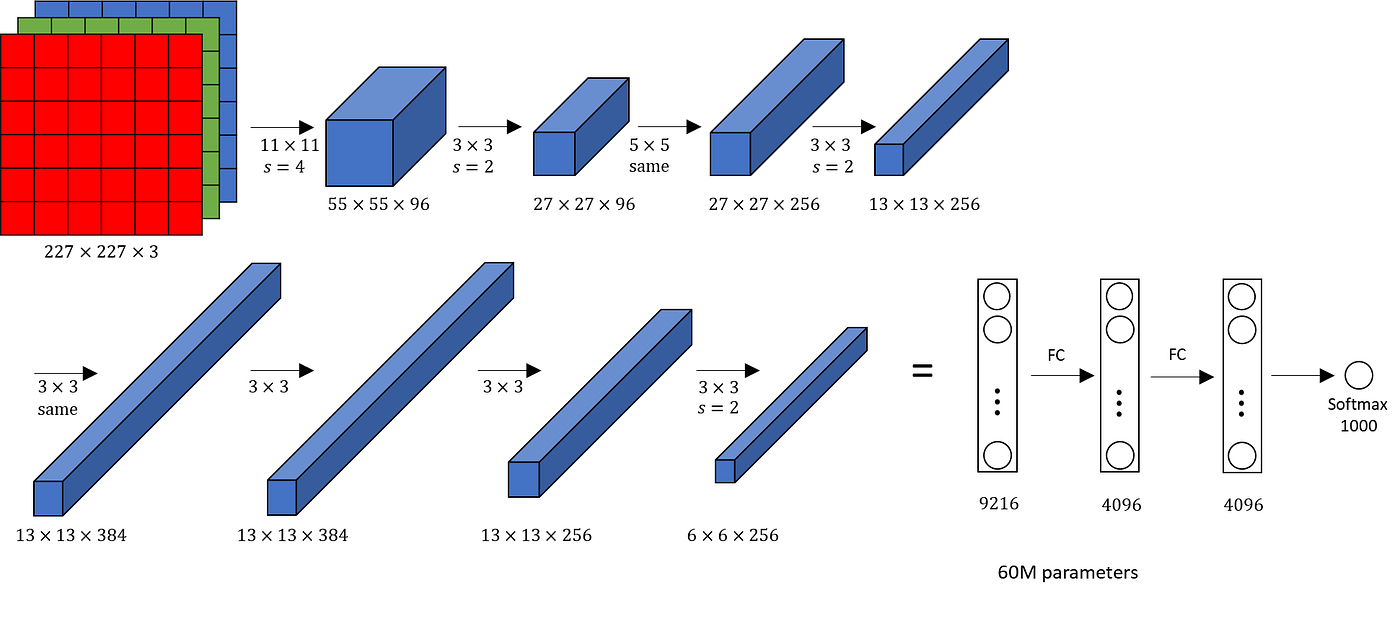
\includegraphics[width=1.0\textwidth]{images/alexnet_architecture_diagram.png}
	\captionof{figure}{Sơ đồ kiến trúc của AlexNet. Mạng được chia thành hai luồng song song để huấn luyện trên hai GPU. Nó bao gồm 5 lớp tích chập (một số được theo sau bởi các lớp max-pooling) và 3 lớp kết nối đầy đủ.}
	\label{fig:alexnet_architecture}
\end{center}
Mạng nhận đầu vào ảnh kích thước $224 \times 224 \times 3$, 
và sử dụng các tham số sau cho từng lớp chính:
\begin{itemize}
	\item Conv1: 96 kernel kích thước $11 \times 11$, stride 4, theo sau bởi max-pooling $3 \times 3$ (stride 2).
	\item Conv2: 256 kernel $5 \times 5$, padding 2, pooling tương tự.
	\item Conv3–5: 384, 384, 256 kernel $3 \times 3$ (padding 1).
	\item FC6–8: 4096, 4096, và 1000 nơ-ron tương ứng.
\end{itemize}
Tổng cộng, mạng có khoảng \textbf{60 triệu tham số} và thực hiện khoảng 650 nghìn phép nhân chập trên mỗi ảnh đầu vào.


\subsubsection{Những Đột phá Kỹ thuật then chốt}
\label{subsubsec:alexnet_innovations}
Thành công của AlexNet không chỉ đến từ việc nó "sâu" hơn, mà chủ yếu đến từ việc kết hợp một cách thông minh các kỹ thuật mới (vào thời điểm đó) để giải quyết các vấn đề cố hữu trong việc huấn luyện mạng sâu.

\begin{description}
	\item[Hàm kích hoạt ReLU:] Đây là một trong những đóng góp quan trọng nhất. Thay vì các hàm Tanh hay Sigmoid vốn gây ra vấn đề suy giảm gradient, AlexNet là kiến trúc quy mô lớn đầu tiên sử dụng thành công hàm \textbf{Rectified Linear Unit (ReLU)}. Với đạo hàm bằng 1 cho các giá trị dương, ReLU cho phép gradient lan truyền ngược qua nhiều lớp mà không bị yếu đi, giúp mạng huấn luyện nhanh hơn đáng kể (tác giả báo cáo là nhanh hơn gấp 6 lần so với Tanh).
	
	\paragraph{Trực giác:} 
	Hàm ReLU ($f(x) = \max(0, x)$) cắt bỏ toàn bộ giá trị âm, chỉ giữ lại các kích hoạt dương. 
	Điều này tạo ra hiện tượng “kích hoạt thưa thớt” (\textit{sparse activation}) — 
	chỉ một phần nhỏ nơ-ron được kích hoạt tại mỗi thời điểm, 
	giúp mạng vừa giảm tương quan giữa các nơ-ron, vừa hội tụ nhanh và ổn định hơn.
	
	
	\item[Kỹ thuật Dropout:] Để chống lại overfitting, một vấn đề nghiêm trọng trong các mạng lớn với hàng chục triệu tham số, AlexNet đã tiên phong sử dụng \textbf{Dropout}. Trong quá trình huấn luyện, tại mỗi bước, Dropout sẽ ngẫu nhiên "tạm thời xóa" một tỷ lệ (ví dụ: 50\%) các nơ-ron trong các lớp kết nối đầy đủ. Điều này buộc các nơ-ron phải học các đặc trưng mạnh mẽ hơn, không thể phụ thuộc vào sự tồn tại của các nơ-ron lân cận. Nó hoạt động như một hình thức "ensemble" nhiều kiến trúc mạng khác nhau, giúp cải thiện đáng kể khả năng tổng quát hóa.
	
	\begin{center}
		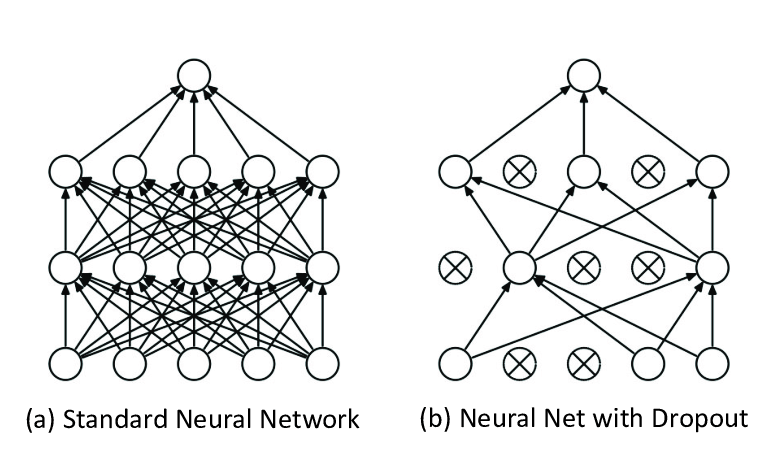
\includegraphics[width=0.6\textwidth]{images/dropout_illustration.png}
		\captionof{figure}{Minh họa kỹ thuật Dropout. (Trái) Một mạng kết nối đầy đủ. (Phải) Cùng mạng đó sau khi áp dụng Dropout, một số nơ-ron và kết nối của chúng bị tạm thời loại bỏ.}
		\label{fig:dropout_illustration}
	\end{center}
	% Keyword gợi ý: dropout neural network illustration, dropout regularization
	
	\item[Tăng cường Dữ liệu (Data Augmentation):] Để làm cho bộ dữ liệu 1.2 triệu ảnh của ImageNet trở nên "lớn" hơn nữa và giúp mạng học được tính bất biến, các tác giả đã áp dụng các kỹ thuật tăng cường dữ liệu một cách mạnh mẽ, bao gồm: cắt cúp ảnh ngẫu nhiên (random cropping), lật ảnh theo chiều ngang (horizontal flipping), và thay đổi cường độ màu sắc của ảnh (PCA color augmentation).
	
	\item[Huấn luyện trên nhiều GPU:] Với 60 triệu tham số, AlexNet quá lớn để có thể chứa vừa trong bộ nhớ của một GPU thời đó (NVIDIA GTX 580 chỉ có 3GB VRAM). Các tác giả đã thực hiện một kỹ thuật song song hóa mô hình, chia mạng thành hai nửa và huấn luyện trên hai GPU riêng biệt, với sự trao đổi thông tin ở một vài lớp nhất định. Đây là một kỳ công kỹ thuật, mở đường cho việc huấn luyện các mô hình ngày càng lớn hơn.
\end{description}

\subsubsection{Kết quả và Tầm ảnh hưởng}
AlexNet không chỉ chiến thắng; nó đã tạo ra một tiêu chuẩn mới.
\begin{table}[h!]
	\centering
	\caption{Kết quả nổi bật tại ILSVRC 2012}
	\label{tab:imagenet_2012_results}
	\begin{tabular}{|l|p{6cm}|c|}
		\hline
		\textbf{Đội/Mô hình} & \textbf{Phương pháp chính} & \textbf{Tỷ lệ lỗi Top-5} \\
		\hline
		\textbf{SuperVision (AlexNet)} & \textbf{Mạng Nơ-ron Tích chập sâu} & \textbf{15.3\%} \\
		\hline
		ISI (Vị trí thứ 2) & SIFT + Fisher Vector + Phân loại & 26.2\% \\
		\hline
	\end{tabular}
\end{table}

AlexNet không chỉ mở ra kỷ nguyên mới của thị giác máy tính, 
mà còn đặt nền móng cho các mô hình CNN hiện đại. 
Các mạng kế nhiệm như \textbf{VGGNet (2014)} và \textbf{GoogLeNet (2014)} 
chính là những nỗ lực tiếp nối nhằm mở rộng và tối ưu hóa “bản thiết kế” mà AlexNet khai sinh.


Khoảng cách 10.9 \% là một con số không tưởng trong một cuộc thi học thuật, báo hiệu sự kết thúc của kỷ nguyên đặc trưng thủ công cho các bài toán nhận dạng quy mô lớn. AlexNet đã cung cấp một \textbf{blueprint (bản thiết kế)} cho các thế hệ CNN sau này: xếp chồng các lớp Conv + ReLU, sử dụng Pooling để giảm chiều, và kết thúc bằng các lớp FC có Dropout để phân loại.

\subsection{VGGNet (2014): Sức mạnh của sự Đồng nhất và Chiều sâu}
\label{subsec:vggnet}

Sau thành công của AlexNet, một câu hỏi lớn được đặt ra: làm thế nào để cải thiện hiệu năng của CNN? Nhóm nghiên cứu Visual Geometry Group (VGG) tại Đại học Oxford đã đưa ra một giả thuyết đơn giản nhưng cực kỳ mạnh mẽ: \textbf{chiều sâu (depth) là yếu tố then chốt}. Mô hình VGGNet \cite{Simonyan2014} của họ, á quân tại ILSVRC 2014, đã chứng minh giả thuyết này một cách thuyết phục.

Trong khi AlexNet đã khai phá tiềm năng của các mạng nơ-ron sâu, 
VGGNet thể hiện bước tiến về \textbf{tính hệ thống và khả năng tổng quát hóa}. 
Khác với AlexNet vốn có nhiều yếu tố thiết kế thủ công, 
VGGNet được xem như một \textit{“kiến trúc chuẩn mực”} cho CNN: 
đồng nhất, sâu, dễ mở rộng và có khả năng tái sử dụng ở nhiều tác vụ khác nhau.

\subsubsection{Triết lý Thiết kế: Đơn giản hóa và Chuẩn hóa}
\label{subsubsec:vgg_philosophy}
Nếu AlexNet có một kiến trúc khá đặc thù (với các kích thước kernel và stride thay đổi), thì VGG lại theo đuổi một triết lý về sự đồng nhất và thanh lịch:
\begin{itemize}
	\item \textbf{Chỉ sử dụng các kernel tích chập rất nhỏ, kích thước $3 \times 3$ (với stride 1, padding 1).}
	\item \textbf{Chỉ sử dụng max-pooling $2 \times 2$ (với stride 2) để giảm chiều không gian.}
\end{itemize}
Toàn bộ mạng được xây dựng bằng cách xếp chồng các "khối" (block) giống hệt nhau, mỗi khối bao gồm 2 hoặc 3 lớp tích chập $3 \times 3$, theo sau là một lớp max-pooling. Cấu trúc này cực kỳ đơn giản, đồng nhất, và dễ dàng mở rộng bằng cách thêm nhiều khối hơn. Các phiên bản phổ biến nhất là \textbf{VGG16} và \textbf{VGG19}, tương ứng với 16 và 19 lớp có trọng số.

\paragraph{Trực giác thiết kế:} 
Việc sử dụng duy nhất kernel $3 \times 3$ không chỉ giúp mạng “gọn” và dễ huấn luyện, 
mà còn đóng vai trò như một \textit{bộ trích chọn vi mô} (micro feature extractor), 
cho phép mô hình học dần các mẫu hình phức tạp từ các cấu trúc nhỏ nhất. 
Đây là triết lý \textbf{“deep and narrow”} – sâu nhưng mỗi lớp chỉ nắm bắt một lượng nhỏ thông tin, 
tạo ra khả năng biểu diễn phân cấp rất mạnh.

\subsubsection{Ưu điểm của việc Chồng các Kernel 3x3}
\label{subsubsec:vgg_3x3_kernels}
Tại sao việc sử dụng nhiều lớp $3 \times 3$ lại tốt hơn một lớp có kernel lớn (ví dụ $5 \times 5$ hoặc $7 \times 7$)?
\begin{enumerate}
	\item \textbf{Tăng tính phi tuyến:} Một chuỗi 3 lớp tích chập có 3 hàm kích hoạt ReLU xen kẽ, trong khi một lớp $7 \times 7$ chỉ có một. Điều này làm cho hàm quyết định có tính phân biệt cao hơn.
	\item \textbf{Giảm số lượng tham số:} Một lớp tích chập $7 \times 7$ trên một input có $C$ kênh sẽ có $7 \times 7 \times C \times C_{out} = 49 \cdot C \cdot C_{out}$ tham số. Trong khi đó, 3 lớp $3 \times 3$ xếp chồng lên nhau sẽ có $3 \times (3 \times 3 \times C \times C_{out}) = 27 \cdot C \cdot C_{out}$ tham số, giảm gần một nửa.
	\item \textbf{Cùng một trường thụ cảm hiệu quả (Effective Receptive Field):} Một chuỗi 3 lớp tích chập $3 \times 3$ có cùng trường thụ cảm hiệu quả như một lớp $7 \times 7$ duy nhất. Tức là, một nơ-ron ở lớp cuối cùng có thể "nhìn" thấy một vùng $7 \times 7$ của input.
\end{enumerate}

Một cách hình thức, trường thụ cảm hiệu quả (\textit{effective receptive field}) $R$ 
của $L$ lớp tích chập kích thước $k \times k$ có thể được ước lượng là:
\begin{equation}
	R = 1 + (k - 1)L
\end{equation}
Với $k=3$ và $L=3$, ta có $R = 7$, tương đương với một lớp $7 \times 7$. 
Công thức này minh họa rõ rằng việc tăng chiều sâu là một cách thay thế hiệu quả 
cho việc dùng kernel lớn, vừa tiết kiệm tham số, vừa tăng phi tuyến.

\begin{center}
	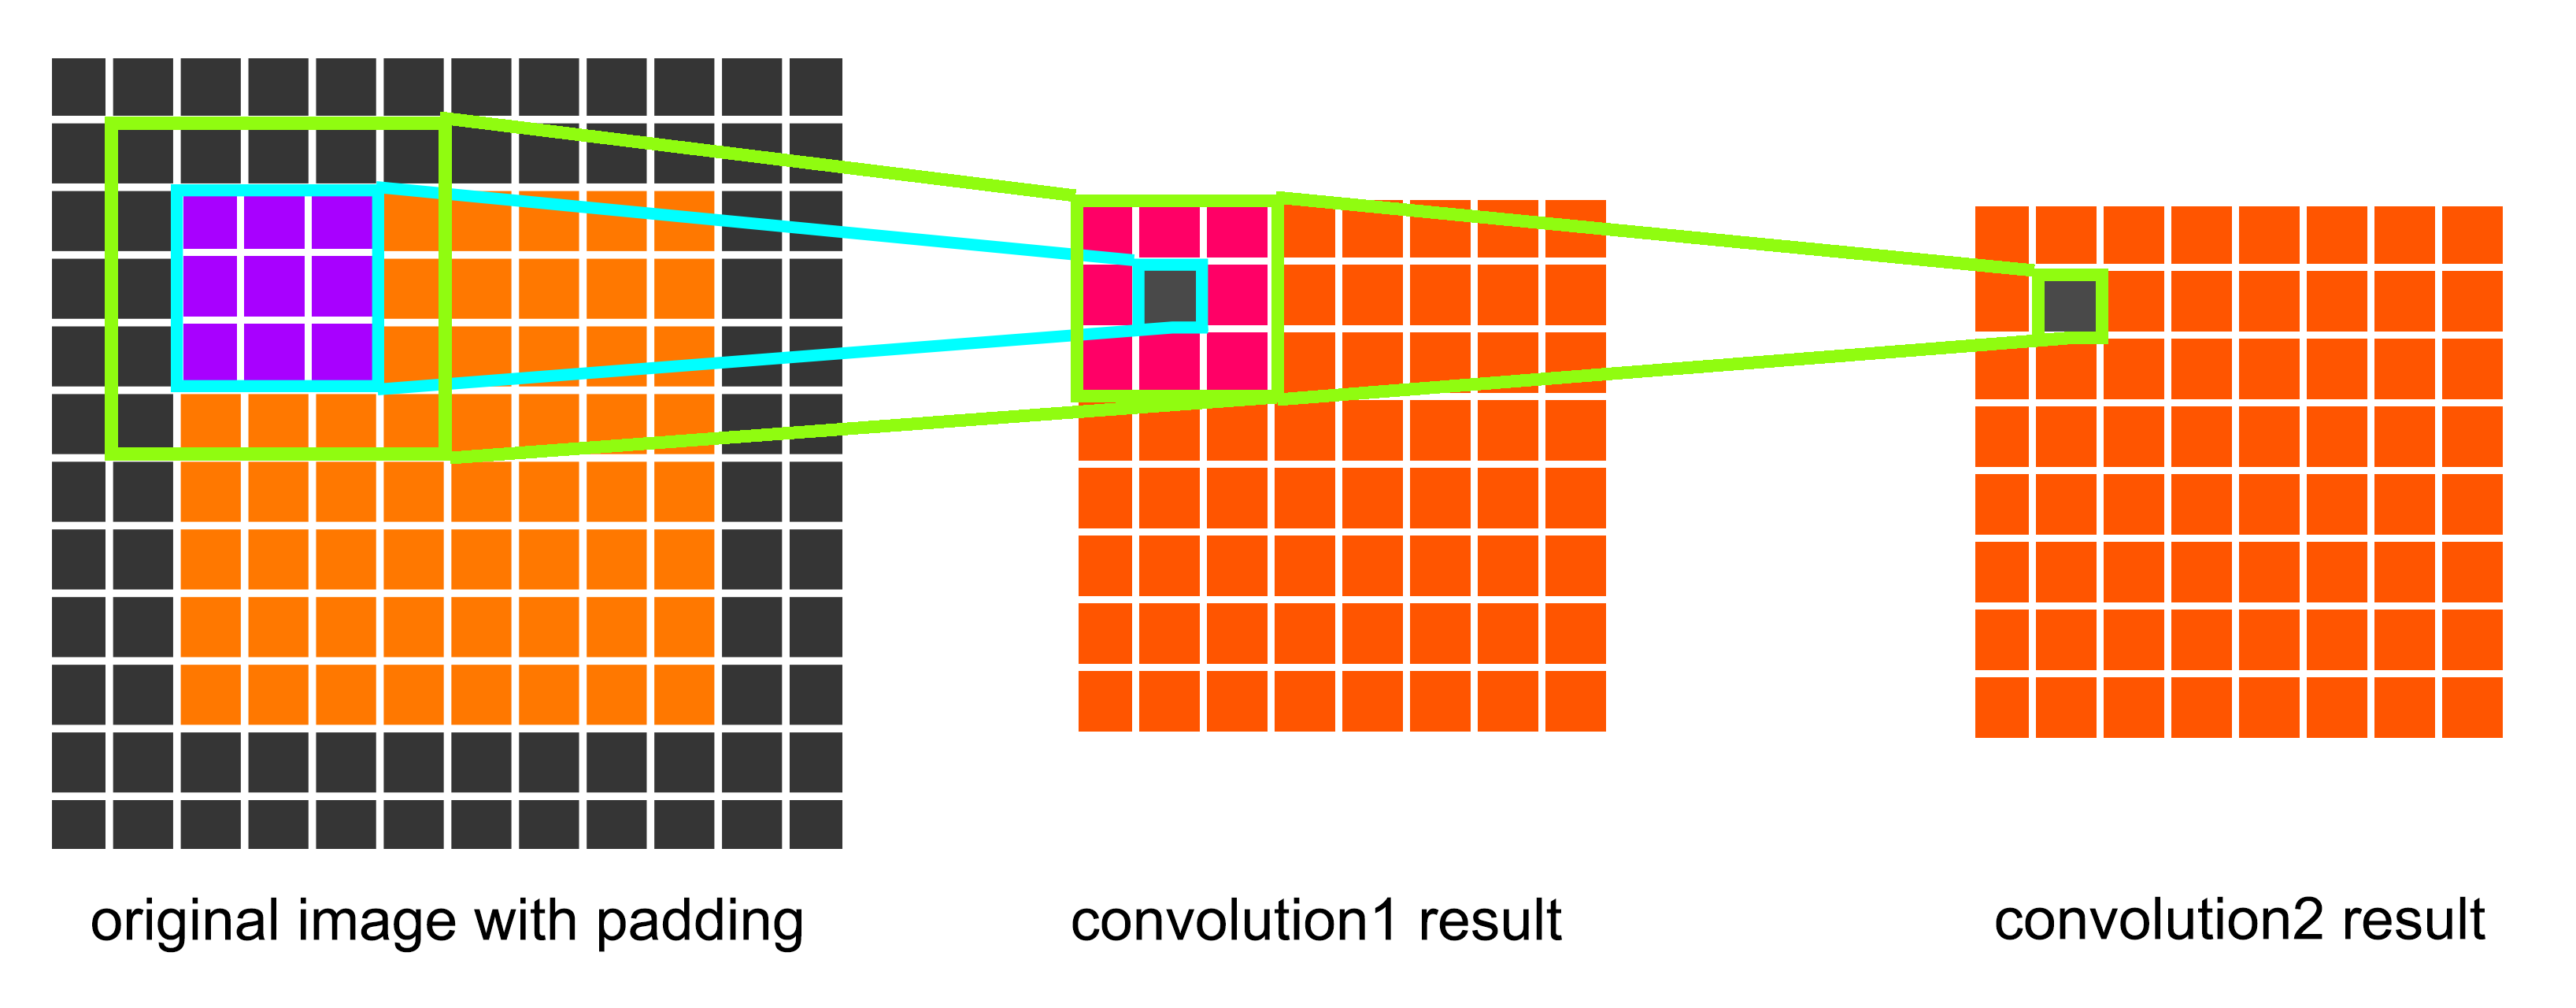
\includegraphics[width=0.7\textwidth]{images/vgg_receptive_field_3x3_stack.png}
	\captionof{figure}{So sánh trường thụ cảm. Một chuỗi 3 lớp tích chập $3 \times 3$ (phải) có cùng trường thụ cảm hiệu quả như một lớp $7 \times 7$ (trái) nhưng với ít tham số hơn và nhiều tính phi tuyến hơn.}
	\label{fig:vgg_receptive_field}
\end{center}
% Keyword gợi ý: vgg receptive field, 3x3 convolution stack

\subsubsection{Kiến trúc VGG16 và Di sản}
VGG16 là một kiến trúc sâu, thẳng và rất mạnh mẽ. Tuy nhiên, điểm yếu lớn nhất của nó là số lượng tham số khổng lồ (khoảng 138 triệu), chủ yếu tập trung ở các lớp kết nối đầy đủ đầu tiên. Điều này làm cho mô hình rất nặng và chậm.

Mặc dù vậy, VGG đã để lại một di sản to lớn. Do cấu trúc đồng nhất và các bản đồ đặc trưng chất lượng cao, các mạng VGG được huấn luyện trước trên ImageNet đã trở thành \textbf{backbone (xương sống)} tiêu chuẩn cho vô số các bài toán khác trong nhiều năm, như phát hiện vật thể (Faster R-CNN), phân đoạn ảnh, và truyền tải phong cách (style transfer).

\begin{center}
	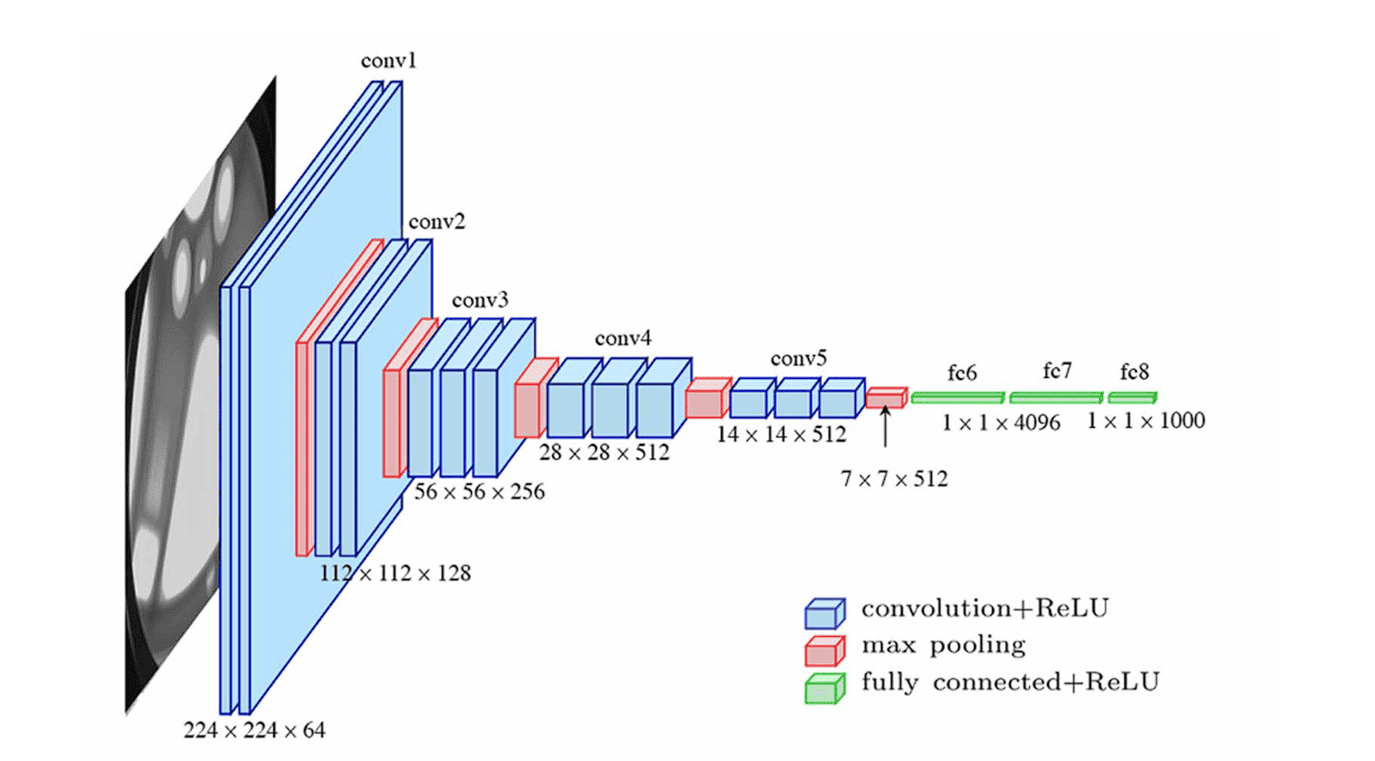
\includegraphics[width=1.0\textwidth]{images/vgg16_architecture_diagram.png}
	\captionof{figure}{Sơ đồ kiến trúc của VGG16. Các khối tích chập $3 \times 3$ và max-pooling được xếp chồng lên nhau, theo sau là các lớp kết nối đầy đủ và một lớp softmax.}
	\label{fig:vgg16_architecture}
\end{center}

\subsection{GoogLeNet (2014): Mạng Inception và Hiệu quả Tính toán}
\label{subsec:googlenet}

Cùng thời điểm với VGG năm 2014, nhóm nghiên cứu của Google (Szegedy et al.) đã giới thiệu một kiến trúc CNN mang tính cách mạng: \textbf{GoogLeNet} (còn gọi là \textbf{Inception v1}) \cite{Szegedy2015}. Nếu VGG chứng minh rằng \textit{“sâu hơn là tốt hơn”}, thì GoogLeNet chứng minh rằng \textit{“thông minh hơn cũng quan trọng không kém”}.  
Thay vì tăng chiều sâu một cách mù quáng, GoogLeNet tập trung vào việc \textbf{tăng hiệu quả sử dụng tham số và tài nguyên tính toán}, giúp mô hình đạt hiệu năng vượt trội mà vẫn tiết kiệm bộ nhớ.

\subsubsection{Động lực Thiết kế}
\label{subsubsec:googlenet_motivation}
Khi các mạng CNN ngày càng sâu hơn (như VGG với hơn 130 triệu tham số), việc huấn luyện trở nên đắt đỏ và dễ dẫn đến overfitting. Nhóm nghiên cứu Google đặt ra câu hỏi:
\begin{quote}
	\textit{“Làm thế nào để mở rộng mạng CNN theo cả chiều sâu và chiều rộng mà không làm tăng quá nhiều tham số?”}
\end{quote}
Câu trả lời là khái niệm \textbf{Inception module} — một “khối” nhỏ gọn nhưng mạnh mẽ, có khả năng trích xuất đặc trưng ở nhiều thang kích thước khác nhau trong cùng một tầng.

\subsubsection{Inception Module: Trích xuất Đặc trưng Đa tỉ lệ}
\label{subsubsec:inception_module}
Thay vì chọn một kích thước kernel cố định (như $3 \times 3$ hoặc $5 \times 5$), GoogLeNet sử dụng đồng thời nhiều kích thước khác nhau:
\begin{itemize}
	\item Nhánh 1: tích chập $1 \times 1$ (giảm chiều kênh và giữ đặc trưng cục bộ).
	\item Nhánh 2: tích chập $3 \times 3$ (nắm bắt đặc trưng trung bình).
	\item Nhánh 3: tích chập $5 \times 5$ (nắm bắt đặc trưng quy mô lớn).
	\item Nhánh 4: pooling $3 \times 3$ (tổng hợp thông tin khái quát).
\end{itemize}
Kết quả từ bốn nhánh này được \textbf{ghép kênh (concatenate)} lại để tạo ra đầu ra của khối Inception.

\begin{center}
	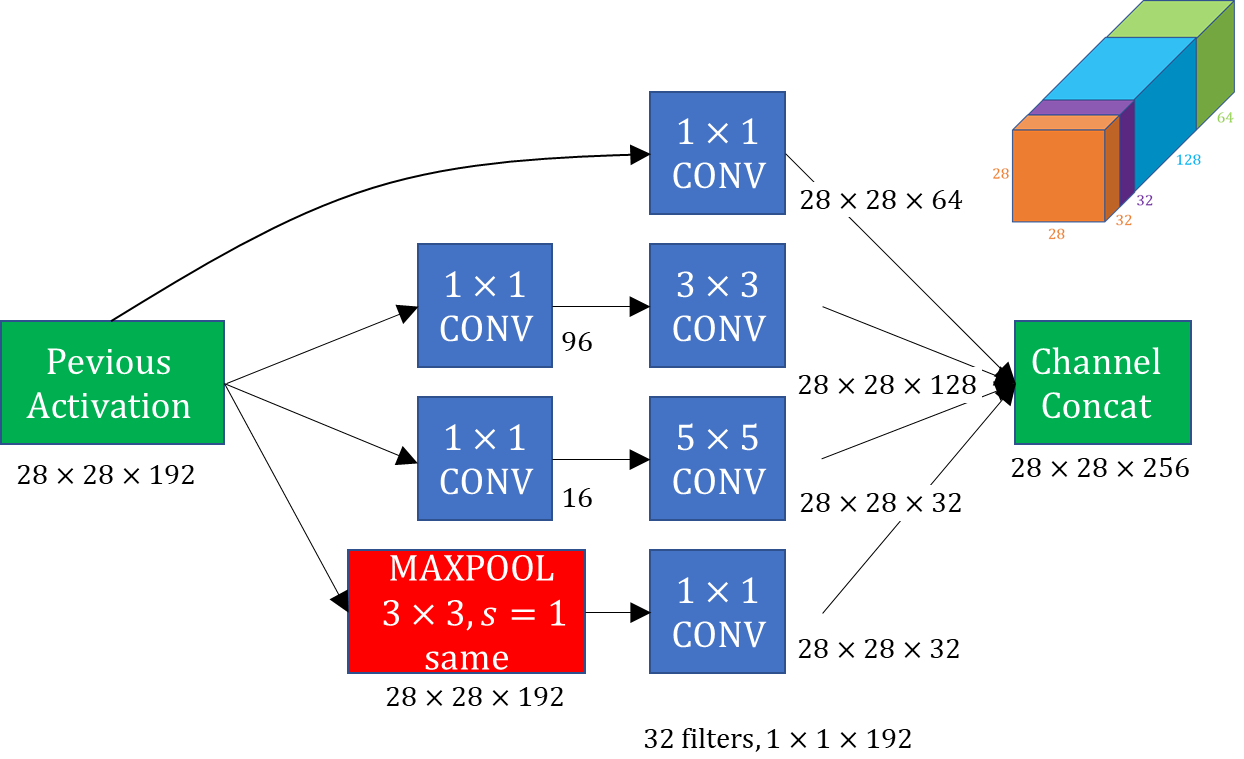
\includegraphics[width=0.8\textwidth]{images/inception_module_diagram.png}
	\captionof{figure}{Cấu trúc của một Inception module trong GoogLeNet. Các nhánh song song sử dụng tích chập kích thước khác nhau và được nối lại theo chiều kênh.}
	\label{fig:inception_module}
\end{center}
% Keyword gợi ý: inception module diagram, googlenet block architecture

\textbf{Điểm sáng tạo quan trọng:}  
Các tích chập $1 \times 1$ được dùng trước các tích chập $3 \times 3$ và $5 \times 5$ để \textbf{giảm số lượng kênh đầu vào} – từ đó giảm mạnh số tham số và chi phí tính toán, mà vẫn giữ được khả năng biểu diễn mạnh mẽ.

\subsubsection{Kiến trúc Tổng thể}
\label{subsubsec:googlenet_architecture}
GoogLeNet gồm 22 lớp có trọng số (khi tính cả các lớp tích chập và fully-connected), nhưng tổng số tham số chỉ khoảng \textbf{5 triệu} – ít hơn gần 30 lần so với VGG16.  
Cấu trúc gồm:
\begin{itemize}
	\item Các lớp tích chập và pooling ban đầu để giảm kích thước không gian.
	\item 9 khối Inception xếp chồng lên nhau.
	\item Một lớp \textbf{Global Average Pooling} thay cho các lớp Fully Connected truyền thống, giúp giảm overfitting và đơn giản hóa mô hình.
\end{itemize}

Ngoài ra, GoogLeNet còn sử dụng \textbf{các nhánh phụ (auxiliary classifiers)} – hai mạng con được gắn vào giữa mô hình, giúp lan truyền gradient tốt hơn trong quá trình huấn luyện (giải quyết phần nào vấn đề \textit{vanishing gradient}).

\begin{center}
	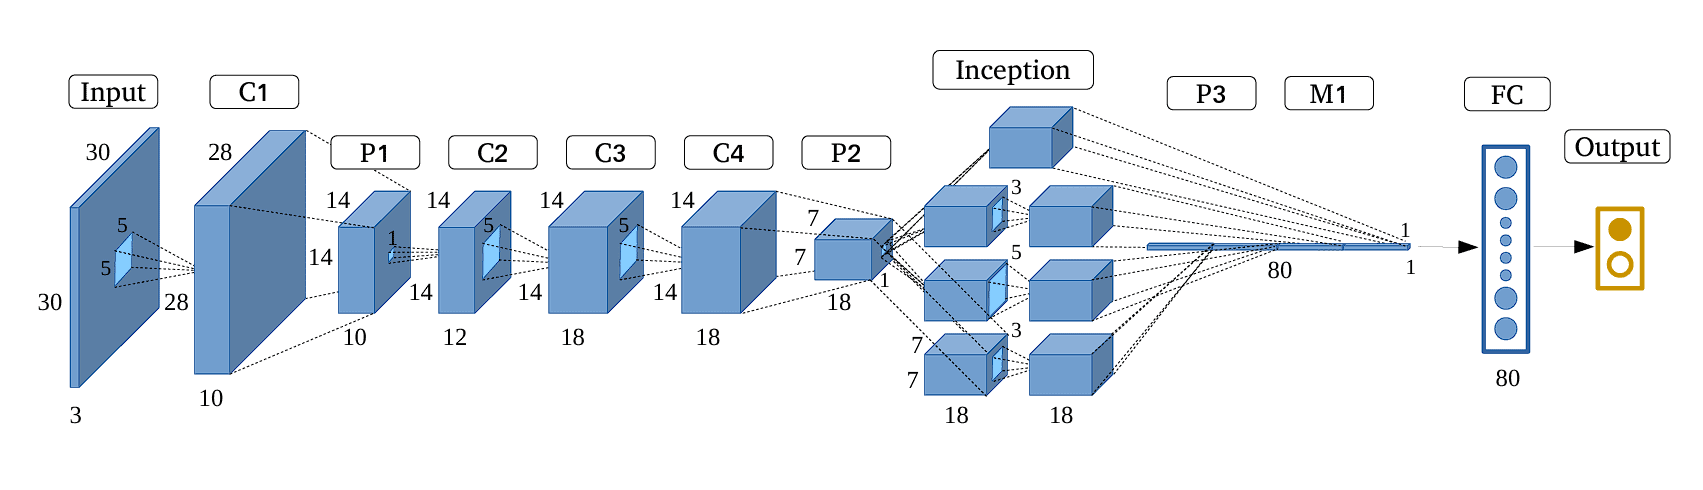
\includegraphics[width=1.0\textwidth]{images/googlenet_architecture_diagram.png}
	\captionof{figure}{Kiến trúc tổng thể của GoogLeNet (Inception v1). Mạng bao gồm 9 khối Inception, xen kẽ giữa các tầng pooling, cùng hai nhánh phụ hỗ trợ huấn luyện.}
	\label{fig:googlenet_architecture}
\end{center}
% Keyword gợi ý: googlenet architecture diagram, inception v1 structure

\subsubsection{Kết quả và Ảnh hưởng}
\label{subsubsec:googlenet_results}
GoogLeNet đã giành chiến thắng tại \textbf{ILSVRC 2014} với tỷ lệ lỗi Top-5 chỉ \textbf{6.7\%}, vượt xa VGG (7.3\%) và giảm gần một nửa so với AlexNet (15.3\%).  
Thành công này không chỉ đến từ độ sâu, mà còn từ triết lý thiết kế hiệu quả, mở đường cho hàng loạt biến thể sau này: Inception v2, v3, v4 và Inception-ResNet.

\begin{table}[h!]
	\centering
	\caption{So sánh các mô hình CNN nổi bật (2012–2014)}
	\label{tab:cnn_comparison_2012_2014}
	\begin{tabular}{|l|c|c|c|}
		\hline
		\textbf{Mô hình} & \textbf{Năm} & \textbf{Số tham số} & \textbf{Tỷ lệ lỗi Top-5 (ImageNet)} \\
		\hline
		AlexNet & 2012 & $\sim$60 triệu & 15.3\% \\
		VGG16 & 2014 & $\sim$138 triệu & 7.3\% \\
		\textbf{GoogLeNet (Inception v1)} & \textbf{2014} & \textbf{$\sim$5 triệu} & \textbf{6.7\%} \\
		\hline
	\end{tabular}
\end{table}

\subsubsection{Di sản của GoogLeNet}
GoogLeNet đã định hình một hướng thiết kế mới cho mạng nơ-ron tích chập:
\begin{itemize}
	\item Mở ra khái niệm \textbf{mạng “rộng và sâu”} (wide \& deep) với cấu trúc song song.
	\item Giới thiệu \textbf{tích chập $1 \times 1$} như một công cụ mạnh mẽ để giảm chiều và tăng phi tuyến.
	\item Thay thế các lớp fully-connected bằng \textbf{Global Average Pooling}, ảnh hưởng trực tiếp đến các kiến trúc hiện đại như ResNet và MobileNet.
\end{itemize}

Nhờ đó, GoogLeNet trở thành cầu nối quan trọng giữa các kiến trúc CNN “cổ điển” (AlexNet, VGG) và các mạng “rất sâu” sau này như ResNet, Inception-v3, và EfficientNet.

\subsection{Bài học Thiết kế và Cầu nối đến các Mạng Rất sâu}
\label{subsec:lessons_from_classics}

Ba kiến trúc kinh điển — \textbf{AlexNet (2012)}, \textbf{VGGNet (2014)} và \textbf{GoogLeNet (2014)} — đã đặt nền móng cho thời kỳ hoàng kim của mạng nơ-ron tích chập. Mỗi mô hình mang đến một tư tưởng thiết kế khác nhau, nhưng tất cả đều góp phần định hình nên nguyên lý phát triển của các kiến trúc hiện đại sau này.

\subsubsection*{Những bài học thiết kế quan trọng}
\begin{itemize}
	\item \textbf{Chiều sâu là chìa khóa (Depth Matters):}  
	AlexNet và đặc biệt là VGG cho thấy rằng việc tăng độ sâu của mạng giúp mô hình học được các đặc trưng phân cấp, từ đơn giản đến phức tạp, dẫn đến hiệu năng vượt trội.
	
	\item \textbf{Đơn giản và đồng nhất giúp mở rộng dễ dàng:}  
	Triết lý thiết kế của VGG — chỉ dùng kernel $3 \times 3$ và cấu trúc khối lặp lại — chứng minh rằng một kiến trúc đơn giản, có quy luật rõ ràng, dễ dàng được nhân rộng và tái sử dụng trong nhiều bài toán khác nhau.
	
	\item \textbf{Hiệu quả tính toán là yếu tố sống còn:}  
	GoogLeNet nhấn mạnh rằng không chỉ độ sâu, mà \textit{tính hiệu quả} trong việc sử dụng tham số và tài nguyên cũng cực kỳ quan trọng. Việc sử dụng tích chập $1 \times 1$ và các khối Inception song song đã mở ra hướng đi mới: mô hình “rộng và sâu” (wide \& deep) nhưng tiết kiệm.
	
	\item \textbf{Regularization và Data Augmentation là bắt buộc:}  
	Các kỹ thuật như Dropout (AlexNet) và tăng cường dữ liệu (AlexNet, GoogLeNet) trở thành thành phần không thể thiếu trong huấn luyện mạng sâu, giúp cải thiện khả năng tổng quát hóa.
	
	\item \textbf{Thay thế các lớp Fully-Connected cồng kềnh:}  
	GoogLeNet giới thiệu \textbf{Global Average Pooling}, thay thế cho các lớp FC nhiều tham số, làm giảm nguy cơ overfitting và đơn giản hóa quá trình suy luận.
\end{itemize}

\subsubsection*{Giới hạn của các kiến trúc cổ điển}
Mặc dù các mạng như VGG và GoogLeNet đã rất sâu so với thời điểm đó (16–22 lớp), khi các nhà nghiên cứu cố gắng đẩy độ sâu lên 30, 50, hay 100 lớp, họ phát hiện ra rằng:
\begin{itemize}
	\item Mạng càng sâu thì quá trình huấn luyện càng khó hội tụ.
	\item Sai số huấn luyện và kiểm thử đều tăng, dù mô hình có khả năng biểu diễn mạnh hơn.
\end{itemize}

Vấn đề cốt lõi không nằm ở overfitting, mà ở hiện tượng \textbf{suy giảm hoặc bùng nổ gradient (vanishing/exploding gradients)} — khi tín hiệu lỗi trong quá trình lan truyền ngược bị yếu dần hoặc tăng vọt, khiến việc tối ưu hóa trở nên bất ổn.

\subsubsection*{Hướng đi mới: Kết nối tắt (Skip Connections)}
Rõ ràng, việc “xếp chồng thêm lớp” không thể mãi là lời giải.  
Cần một cách mới để huấn luyện các mạng \textbf{rất sâu (ultra-deep networks)} mà vẫn ổn định.  
Ý tưởng đột phá đó chính là \textbf{kết nối tắt (residual connections)}, được giới thiệu trong \textbf{ResNet (2015)} — một bước ngoặt giúp mở rộng mạng nơ-ron lên hàng trăm, thậm chí hàng nghìn lớp mà vẫn huấn luyện được.


\section*{Tài liệu tham khảo}
\begin{itemize}
	\item[1] Krizhevsky, A., Sutskever, I.,\& Hinton, G. E. (2012). ImageNet classification with deep convolutional neural networks. In \textit{Advances in neural information processing systems (NIPS)}, 25. (Paper bản lề giới thiệu AlexNet, khởi đầu kỷ nguyên học sâu hiện đại bằng việc chiến thắng ILSVRC 2012 và phổ biến hóa việc sử dụng ReLU, Dropout, và huấn luyện trên GPU).
	\item[2] Simonyan, K.,\& Zisserman, A. (2014). Very deep convolutional networks for large-scale image recognition. \textit{arXiv preprint arXiv:1409.1556}. (Paper giới thiệu kiến trúc VGGNet, nhấn mạnh vai trò của chiều sâu và thiết lập tiêu chuẩn cho việc sử dụng các khối tích chập 3x3 đồng nhất).
	\item[3] LeCun, Y., Bottou, L., Bengio, Y.,\& Haffner, P. (1998). Gradient-based learning applied to document recognition. \textit{Proceedings of the IEEE}, 86(11), 2278-2324. (Paper kinh điển giới thiệu LeNet-5, tiền thân của các kiến trúc CNN hiện đại, cung cấp bối cảnh lịch sử quan trọng).
	\item[4] Russakovsky, O., Deng, J., Su, H., Krause, J., Satheesh, S., Ma, S., ...\& Fei-Fei, L. (2015). ImageNet Large Scale Visual Recognition Challenge. \textit{International Journal of Computer Vision}, \textit{115}(3), 211-252. (Mô tả chi tiết về bộ dữ liệu ImageNet và cuộc thi ILSVRC, "sân khấu" đã làm nên tên tuổi của AlexNet và VGG).
	\item[5] Srivastava, N., Hinton, G., Krizhevsky, A., Sutskever, I.,\& Salakhutdinov, R. (2014). Dropout: a simple way to prevent neural networks from overfitting. \textit{The journal of machine learning research}, 15(1), 1929-1958. (Paper gốc giải thích chi tiết về kỹ thuật Dropout, một thành phần chính giúp AlexNet và các mạng sau này chống lại overfitting).
\end{itemize}